% Generated by tests/contracts/run-request-processing-benchmark.mjs
\begin{table*}[t]
\centering
\caption{Deterministic request-processing benchmark across 4 scenarios. Higher is better for pass rate, lead accuracy, embodied recall, and verification completeness. Lower is better for over-decomposition, forbidden mutation, generative plan collapse, and false completion.}
\label{tab:deterministic-benchmark}
\resizebox{\textwidth}{!}{%
\begin{tabular}{lccccccccc}
\toprule
System & Pass Rate & Lead Top-1 & Recall@3 & Over-Decomp & Forbidden Mutation & Embodied Recall & Collapse & Verification & False Completion \\
\midrule
Direct-Tool & 0.0\% & 0.0\% & 0.0\% & 0.0\% & 100.0\% & 0.0\% & 100.0\% & 27.8\% & 75.0\% \\
Request-Rooted & 100.0\% & 100.0\% & 100.0\% & 0.0\% & 0.0\% & 100.0\% & 0.0\% & 100.0\% & 0.0\% \\
Task-First & 0.0\% & 50.0\% & 100.0\% & 100.0\% & 0.0\% & 66.7\% & 33.3\% & 72.2\% & 0.0\% \\
\bottomrule
\end{tabular}
}
\end{table*}

\begin{figure}[t]
\centering
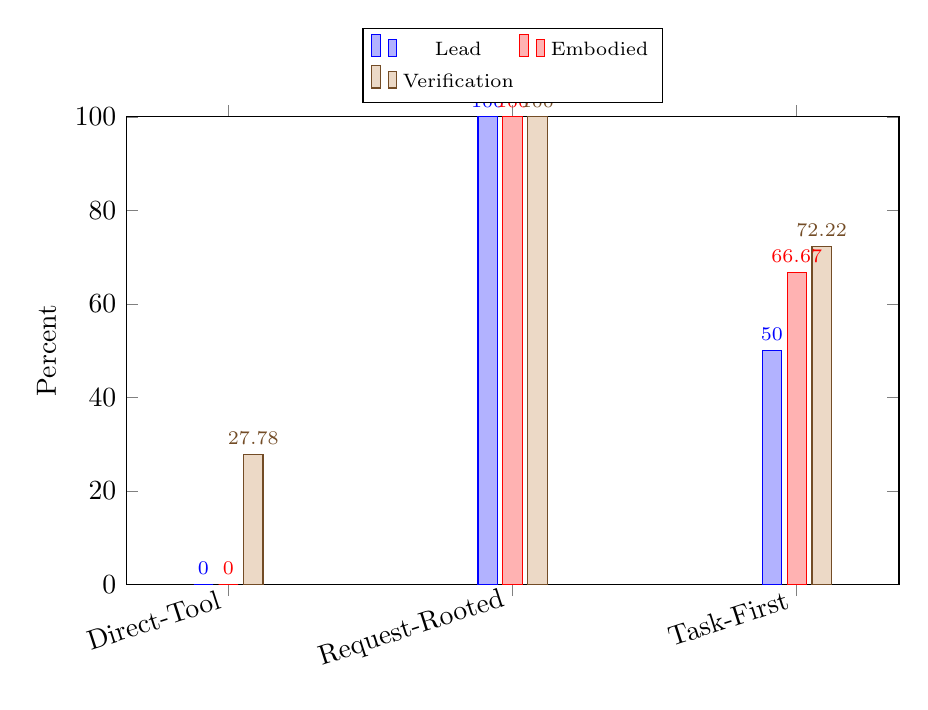
\begin{tikzpicture}
\begin{axis}[
  ybar,
  bar width=7pt,
  width=0.94\columnwidth,
  height=0.62\columnwidth,
  ymin=0,
  ymax=100,
  ylabel={Percent},
  symbolic x coords={Direct-Tool,Request-Rooted,Task-First},
  xtick=data,
  x tick label style={rotate=18, anchor=east},
  legend style={font=\scriptsize, at={(0.5,1.03)}, anchor=south, legend columns=2},
  nodes near coords,
  every node near coord/.append style={font=\scriptsize},
  enlarge x limits=0.18
]
\addplot coordinates {(Direct-Tool, 0) (Request-Rooted, 100) (Task-First, 50)};
\addplot coordinates {(Direct-Tool, 0) (Request-Rooted, 100) (Task-First, 66.66666666666666)};
\addplot coordinates {(Direct-Tool, 27.777777777777775) (Request-Rooted, 100) (Task-First, 72.22222222222221)};
\legend{Lead, Embodied, Verification}
\end{axis}
\end{tikzpicture}
\caption{Outcome quality on the deterministic benchmark. The request-rooted baseline preserves both routing quality and embodied verification fidelity, while the direct-tool baseline collapses on physical-work retention.}
\label{fig:deterministic-benchmark}
\end{figure}
